\section{背景知识}

本章介绍有关AdaptiveLLM的背景知识。由于AdaptiveLLM主要面向LLM推理过程中产生的KV Cache~\cite{KV-Cache}内存占用进行优化,因此本章将在第一节阐明KV Cache在LLM推理任务中的功能,在第二节论述传统工作中面向KV Cache的内存优化技术。

\subsection{KV Cache的提出}

LLM推理任务以token作为输入与输出的基本单位。对于生成式推理任务,每次前向传播计算仅生成一个新token。一般来说,其包含两个阶段:prefill阶段读取用户输入的token序列,生成第一个token;decode阶段分为多步进行,依次生成后续token,直至得到终止token。在推理过程中,每个token拥有一个key-value张量对,为自注意力机制下的编码结果。

\begin{figure}[!htbp]
  \centering
  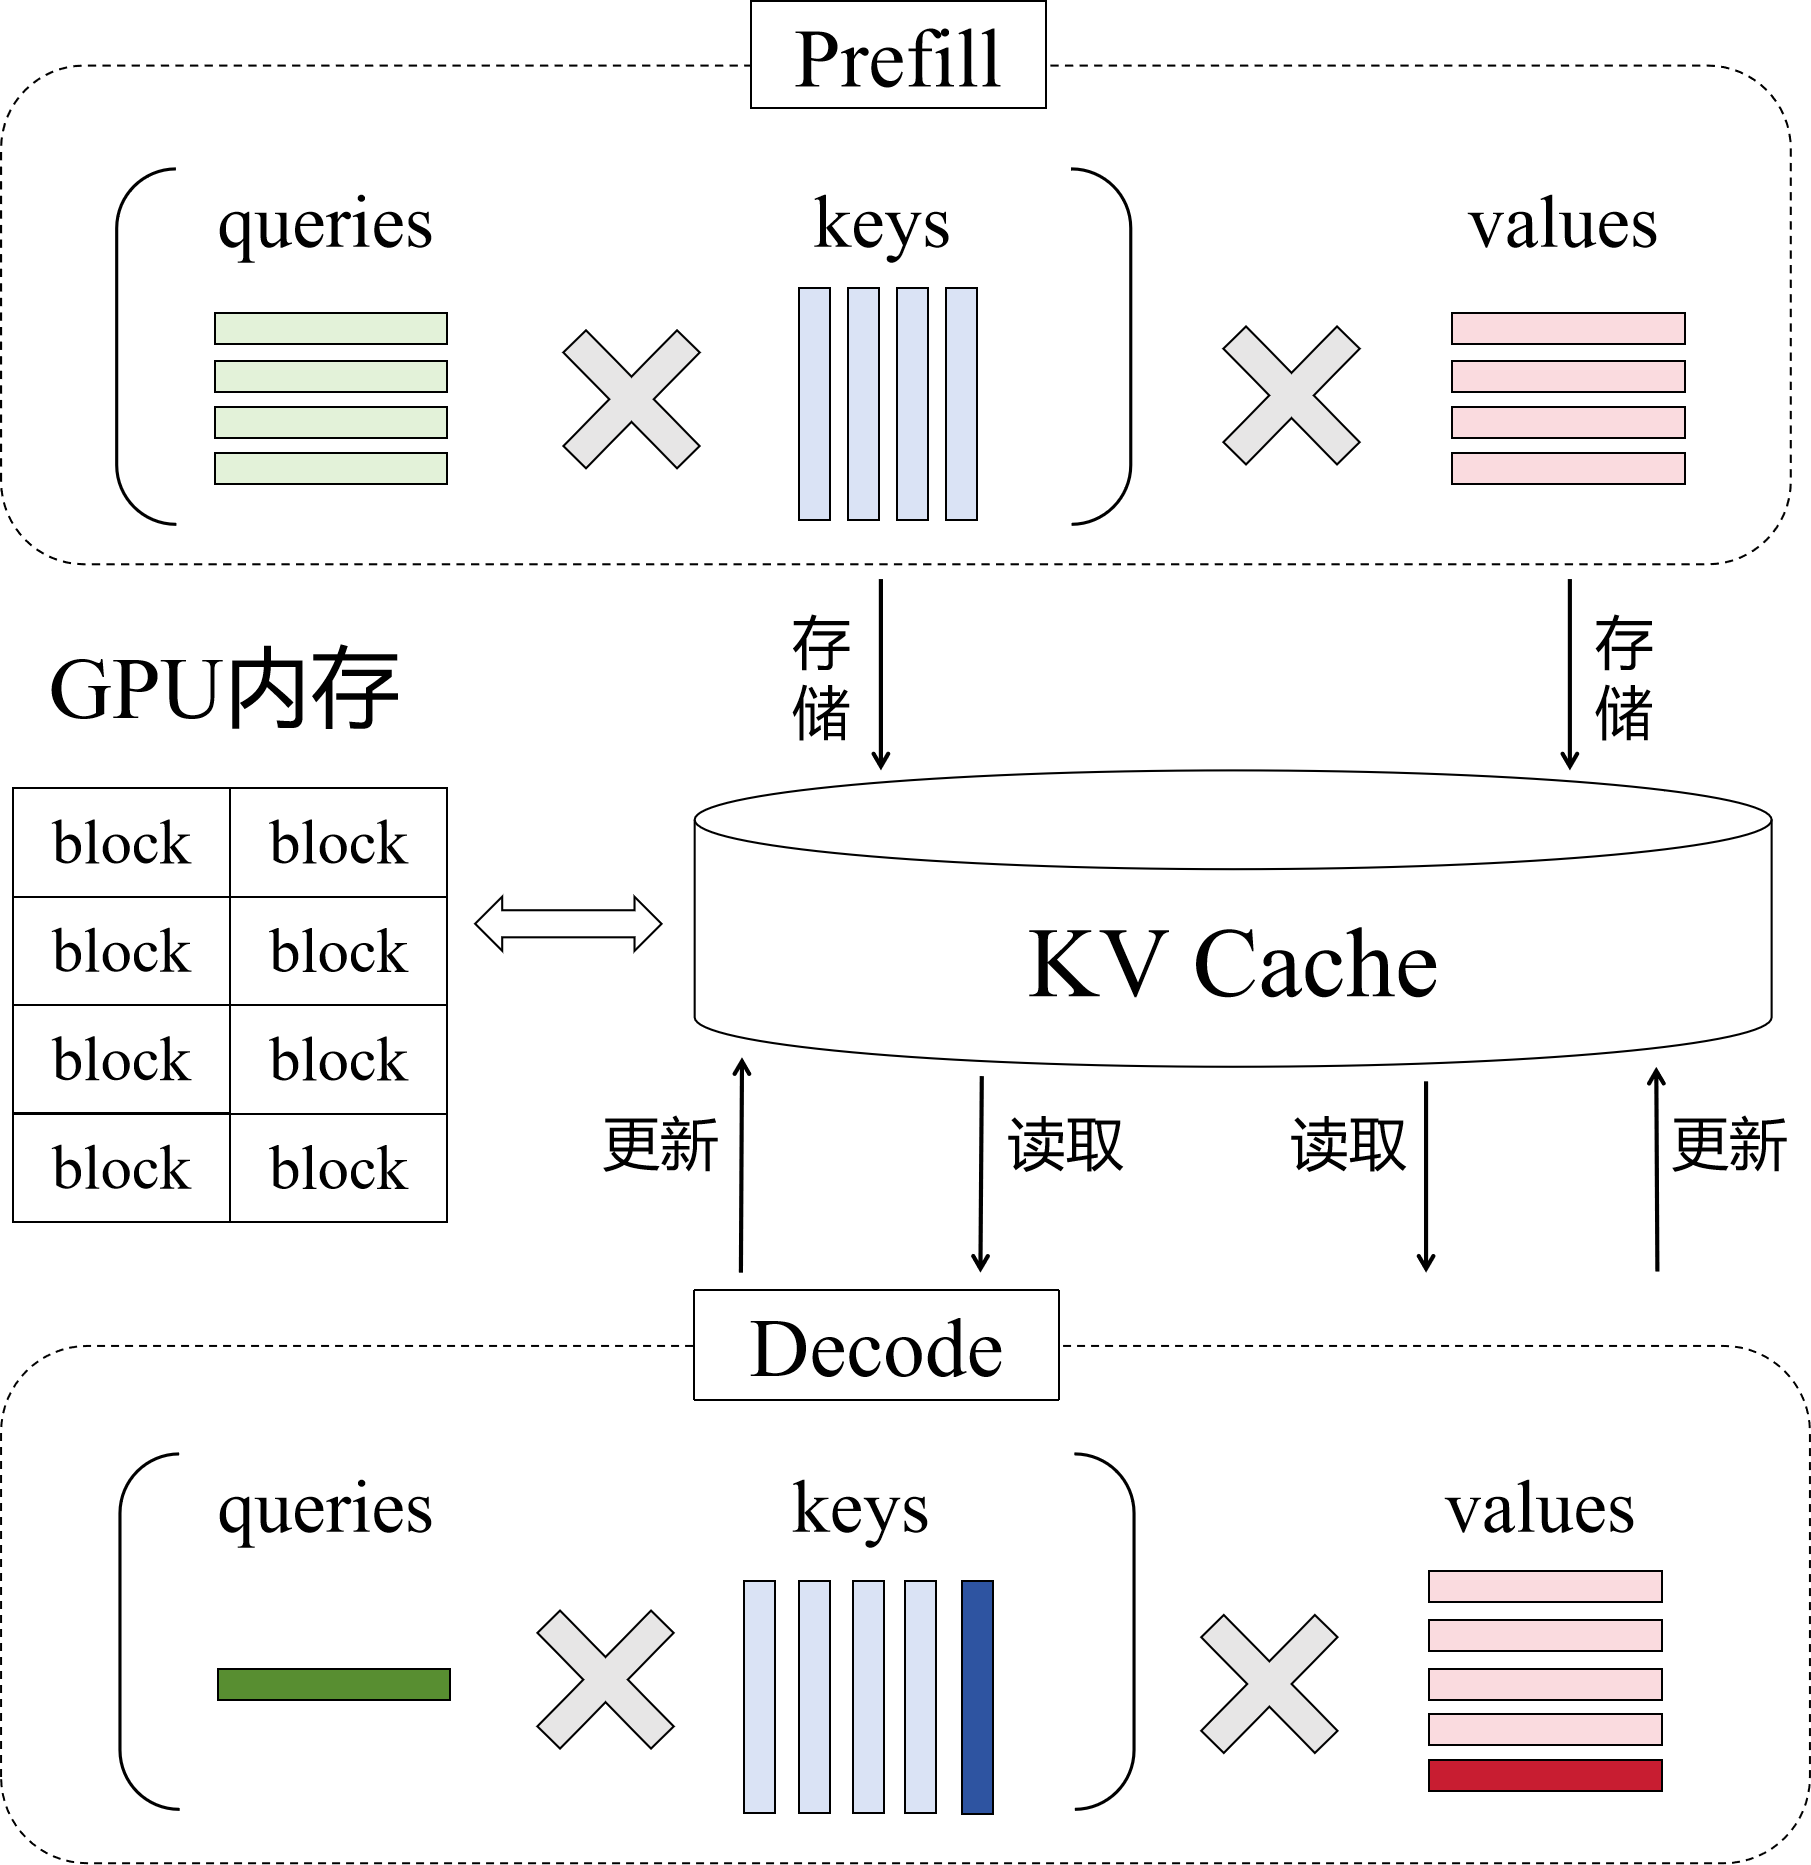
\includegraphics[width=0.8\linewidth]{KV Cache的功能示意图.png}
  \caption{KV Cache的功能示意图}
  \label{Fig:KV Cache的功能示意图}
\end{figure}

在decode阶段中,每个token的计算过程均依赖于前序token的key值和value值。如果每次计算前都重新调用自注意力机制来获取前序token的key-value张量对,则会产生大量不必要的计算开销。目前主流的LLM推理服务~\cite{Swapping, vLLM, ORCA, SpecInfer,SARATHI}框架普遍采用KV Cache数据结构来保存这些token的key-value张量,方便后续token的生成,避免重复计算,减少GPU算力消耗。其工作原理如图\ref{Fig:KV Cache的功能示意图}所示。

然而,随着后续token的不断生成,KV Cache迅速扩展,产生推理内存瓶颈。例如,在OPT-13B模型中,对于一个长度为100的用户请求,其KV Cache能够占用39.1MB的内存空间。有限的GPU内存将批处理大小限制在较低水平,阻碍推理并发度的进一步提升,进而限制吞吐率。

不同于LLM参数张量,KV Cache占用的内存空间在对应用户请求推理完毕后被释放。 其内存占用量大、动态性高,拥有较大的优化空间,因此AdaptiveLLM的内存优化策略将针对KV Cache实现。

\subsection{KV Cache的内存优化}

KV Cache的引入方便了计算过程,却带来内存瓶颈,使得LLM推理性能的提升无法达到预期水平。下面介绍针对KV Cache内存占用的一些优化工作。

\subsubsection{内存碎片优化}

在传统LLM推理服务框架~\cite{Swapping}中,内存管理器按照用户定义的序列长度上限,为每个请求设置一块固定大小的GPU内存来存储KV Cache。但用户请求长度的差异性导致内碎片的大量产生。为了解决该问题,部分LLM推理框架~\cite{Output-Length-Prediction}能够基于历史信息来预测输出长度,并按照预测值分配内存。然而,预测误差会导致输出截断,且旧请求的完成与新请求的加入使得内存中产生很多外碎片。随着新请求的不断到来,内碎片与外碎片在内存中积累,严重影响了内存空间的高效使用。基于这些问题,vLLM框架~\cite{vLLM}引入了Paged Attention机制,基于OS页式内存管理思想,将GPU内存划分成块,并通过维护块表来支持KV Cache在内存空间中的不连续存储。该机制基本消除了内碎片和外碎片现象,大大提升内存利用率。

\subsubsection{张量交换与张量重算}

为了攻克推理内存瓶颈,传统框架引入了张量交换技术~\cite{Swapping, vLLM, LightLLM},将暂时不会使用的KV Cache传输至CPU中,在计算需要时重新传输至GPU中。然而,CPU-GPU间有限的PCIe带宽使得换出和换入过程产生不可忽略的通信开销,限制吞吐率,降低推理性能。部分研究提出~\cite{Recomputation},当张量交换带来的开销超过重新调用自注意力机制的开销时,应选择后者来获取所有前序token的key-value张量,也称张量重算。具体来说,内存管理器直接删除重算请求对应的KV Cache,在其被调度时执行一次prefill阶段来代替原本应该执行的decode阶段。重算与交换的联合使用缓解了通信开销问题,然而,当GPU内存不足时,如何在二者中进行选择成为了新的困境。AdaptiveLLM针对此问题设计了基于开销感知的内存优化策略,能够预测二者的开销,并选择开销小的过程执行。
